\chapter{TCP server}

\section{Opgaveformulering}

Der skal udvikles en server med support for en client ad gangen, som kan modtage
en tekststreng fra en client. Serveren skal køre i en virtuel Linux-maskine.
Tekststrengen skal indeholde et filnavn, eventuel ledsaget af en stiangivelse.
Tilsammen skal informationen i tekststrengen udpege en fil af en vilkårlig
type/størrelse i serveren, som en tilsluttet client ønsker at hente fra serveren. Hvis
filen ikke findes skal serveren returnere en fejlmelding til client’en. Hvis filen findes
skal den overføres fra server til client i segmenter på 1000 bytes ad gangen – indtil
filen er overført fuldstændigt. Serverens portnummer skal være 9000. Serverapplikationen
skal kunne startes fra en terminal med kommandoen:\\ \\
\#./file\_server (for C/C++ applikationers vedkommende)\\
\#./file\_server.exe (for C\# applikationers vedkommende)\\
\#python file\_server.py (for Python applikationers vedkommende)\\ \\
Serveren skal være iterativ, dvs. den skal ikke lukke ned når den har sendt en fil til en
client. Den skal, efter endt filoverførsel, kunne håndtere en ny forespørgsel fra en
client (samme client eller en anden client).
Serveren skal kun kunne håndtere en client ad gangen.

\section{TCP server}

TCP er en protokol som er pålidelig, da den opretter en fast forbindelse mellem server og klient, ved et såkaldt "handshake", før en overførsel initieres. 
Det vil sige, at så snart en TCP forbindelse er oprettet, vil pakkerne der sendes ikke længere have brug for en modtager-adresse, men kan blot "dumpes" ned i den TCP-strøm som løber imellem klient og server. 
TCP benytter desuden også ordnet levering dvs. pakkerne ankommer til modtageren i samme rækkefølge som de blev afsendt.

Vi starter med at oprette en socket for at kunne kommunikere med clienten. \\

\begin{lstlisting}
sock = socket(AF_INET, SOCK_STREAM, 0);
\end{lstlisting}

Vi binder serverens adresse og portnummer til socket'en. Vi benytter et fast portnummer som er 9000, for at gøre det lettere. 

Herefter venter serveren på at clienten tager kontakt til serveren ved hjælp af TCP. Når clienten tager kontakt til serveren oprettes en socket til den indkommende forbindelse. 

\begin{lstlisting}
newsock = accept(sock, (struct sockaddr *) &cli_addr, &client_size);
\end{lstlisting}

Herefter afventer serveren at clienten sender filnavnet, som clienten ønsker at hente fra serveren. Serveren læser filnavnet fra clienten ved hjælp af funktionen \textit{readTextTCP()} fra det udleverede bibliotek LIB. 

Hvis filen eksisterer kaldes funktionen \textit{sendFile()} ellers sender serveren en fejlmeddelse til clienten og lukker forbindelsen. 

I det efterfølgende vil vi beskrive funktionen \textit{sendFile}. 

Når serveren skal sende den efterspurgte fil. Starter vi med at sende filstørrelsen til clienten med TCP, således at clienten ved hvor mange byte den skal modtage. 

Vi opretter en stream og åbner herefter den efterspurgte fil. Open funktionen tager to parametre et char array med filnavnet og flags som specificere om det er input eller output og hvilken operation vi benytter. 

\begin{lstlisting}
std::ifstream FileIn; 
FileIn.open(fileName.c_str(), std::ios::in | std::ios::binary);
\end{lstlisting}

Da vores filnavn er en string benytter vi c++ funktinen \textit{c\_str()} til konvertere strengen om til et char array. Vi har angivet at det er et input og at filen skal sendes i binære mode, hvilket var et krav til opgaven. 

Vi tjekker for om filen eksisterer og om den er blevet åbnet korrekt.
Hvis dette er tilfældet begynder vi at sende data til clienten. Dette gør vi ved at oprette en variabel kaldet rest som indeholder filstørrelsen. 
I et while-loop tester vi for om rest er større end 0 dvs. om der er mere data der skal sendes. 
Vi læser herefter 1000 bytes fra filen ved hjælp af funktionen \textit{redsome()}. Denne funktion returnerer hvor mange bits der er blevet læst, hvilket vi benytter så vi ved hvor mange bits vi skal sende til clienten. Vi kan nemlig være sikker på at der altid vil blive læst til 1000 bytes. 
Herefter tester vi for om vi har læst nogen data, hvis dette ikke er tilfældet forsøger vi igen. Hvis det er tilfældet sender vi dataerne vi har læst til clienten og tæller rest ned. 

\begin{lstlisting}
long rest = fileSize;
while (rest > 0)
{
	int count = FileIn.readsome(buffer,bufferSize); // Reading file 
	if(count >= 0)
	{
		write(outToClient, buffer, count); // sending file
		rest -= count;
	}
}
\end{lstlisting}

\clearpage
Princippet ovenfor kan beskrives med følgende figur. 
\begin{figure}[h]
\centering
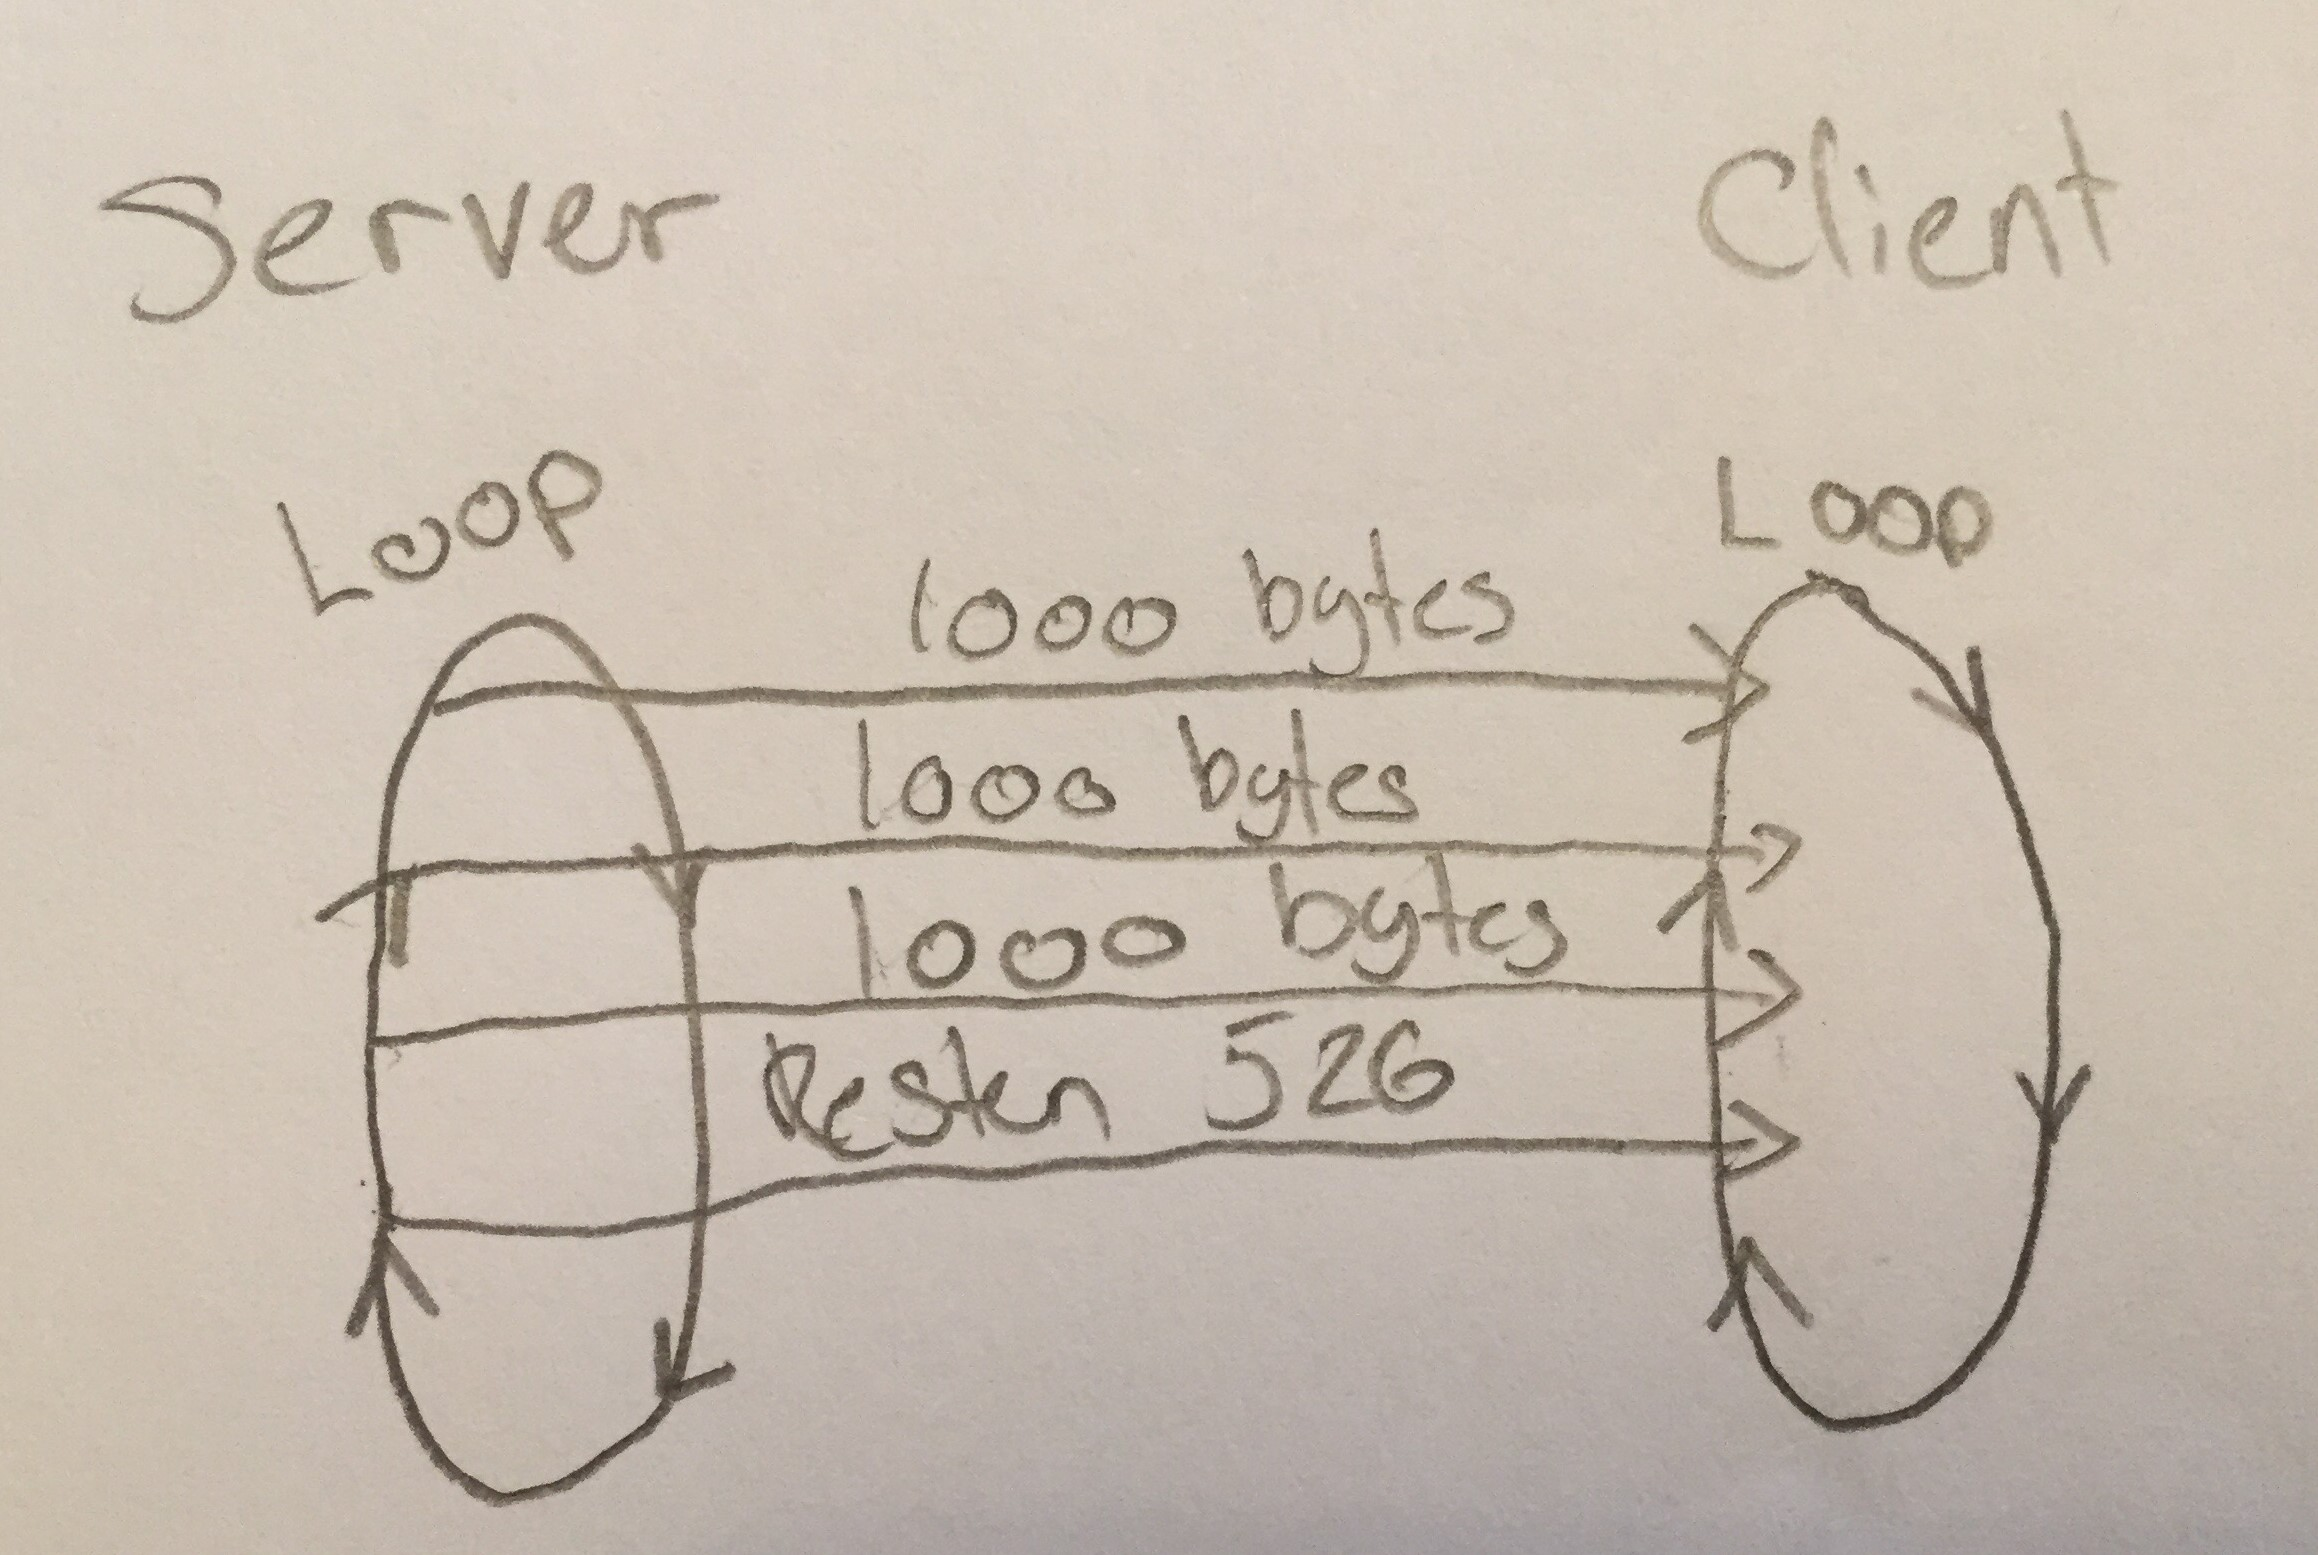
\includegraphics[width=0.7\linewidth]{Pic/Loop}
\caption{Loop 1000 bytes}
\label{fig:Loop}
\end{figure}

Her ses at serveren sender 1000 bytes af gangen og når der er mindre end 1000 bytes tilbage sendes resten. 


